% answers.tex —— 1977 年·山西卷 · 参考答案与详细解析片段
% 由 tools/generate_projects.py 依来源总账自 1977/1977_数学真题_山西_试题.md + 1977/1977_数学真题_山西_解析正文.md + 1977/1977_数学真题_山西_答案要点.md 生成，勿手改（改源 MD 后重跑）


\begin{gktip}
固定源是题面与解答连续出现的《山西1977年高考数学试题解》（书籍页码 36—39）。下文逐题对照源解答并重新计算关键结论，各题最终结论与源解答一致。原卷第 2 题三个小题的“1．2．3．”编号已按本库小问连续编号规范重排为（1）（2）（3）；第 2(1) 题原卷把后两个换底因子的真数排印为上标位置，已按源解答确认语义后按真数转录；第 1(2) 题因子 $(b+a)^2$ 中 $b$ 与 $a$ 之间的墨点经 400 dpi 局部放大确认为扫描污渍，字符为加号。原卷函数记号 Lg、Ln、Log、Sin、Cos、tg 在本文件按现代记号展开（lg、ln、log、sin、cos、tan）。
\end{gktip}

\begin{answer}
\gksolhead{1}{}

\textbf{题目}（20 分）：

化简下列各题：

（1） $\dfrac{1}{\sqrt2+1}-\dfrac{1}{\sqrt2-1}$；

（2） $\dfrac{(a^2-b^2)^3}{a^3+b^3}\div\dfrac{(b+a)^2}{a^2-ab+b^2}\times\dfrac{1}{(b-a)^3}$；

（3） $\dfrac{2\operatorname{Lg}6-\operatorname{Lg}3}{1+\frac12\operatorname{Lg}0.36+\frac13\operatorname{Lg}8}$；

（4） $\dfrac{x^4+x^2+1}{x^3-1}+\dfrac{x(x-2)-2(x-2)}{x^2-3x+2}$.

\Needspace{4\baselineskip}
\textbf{解析}

\gksubpart{（1）}

\Needspace{5\baselineskip}
分别把两个分母有理化：

\nopagebreak[4]
\[
\frac{1}{\sqrt2+1}=\frac{\sqrt2-1}{(\sqrt2+1)(\sqrt2-1)}=\frac{\sqrt2-1}{2-1}=\sqrt2-1,
\]

\nopagebreak[4]
\[
\frac{1}{\sqrt2-1}=\frac{\sqrt2+1}{(\sqrt2-1)(\sqrt2+1)}=\sqrt2+1.
\]

\Needspace{5\baselineskip}
所以

\nopagebreak[4]
\[
\frac{1}{\sqrt2+1}-\frac{1}{\sqrt2-1}=(\sqrt2-1)-(\sqrt2+1)=-2.
\]

\gksubpart{（2）}

\Needspace{5\baselineskip}
由 $a^2-b^2=(a+b)(a-b)$ 得 $(a^2-b^2)^3=(a+b)^3(a-b)^3$；又 $a^3+b^3=(a+b)(a^2-ab+b^2)$，且 $b+a=a+b$、$b-a=-(a-b)$。于是除法化为乘法：

\nopagebreak[4]
\[
\begin{aligned}
\text{\text{原式}}
&=\frac{(a+b)^3(a-b)^3}{(a+b)(a^2-ab+b^2)}
\cdot\frac{a^2-ab+b^2}{(a+b)^2}\cdot\frac{1}{-(a-b)^3}\\[2pt]
&=(a+b)^2(a-b)^3\cdot\frac{1}{(a+b)^2}\cdot\frac{1}{-(a-b)^3}\\
&=-1.
\end{aligned}
\]

\gksubpart{（3）}

\Needspace{5\baselineskip}
分子：

\nopagebreak[4]
\[
2\lg6-\lg3=\lg6^2-\lg3=\lg36-\lg3=\lg\frac{36}{3}=\lg12.
\]

\Needspace{5\baselineskip}
分母（$\lg10=1$、$\frac12\lg0.36=\lg\sqrt{0.36}=\lg0.6$、$\frac13\lg8=\lg\sqrt[3]{8}=\lg2$）：

\nopagebreak[4]
\[
1+\frac12\lg0.36+\frac13\lg8=\lg10+\lg0.6+\lg2=\lg(10\times0.6\times2)=\lg12.
\]

所以原式 $=\dfrac{\lg12}{\lg12}=1$。

\gksubpart{（4）}

\nopagebreak[4]
\[
x^4+x^2+1=(x^2+1)^2-x^2=(x^2+x+1)(x^2-x+1),
\]

\nopagebreak[4]
\[
x^3-1=(x-1)(x^2+x+1),\qquad
x(x-2)-2(x-2)=(x-2)^2,\qquad
x^2-3x+2=(x-2)(x-1).
\]

\Needspace{5\baselineskip}
因此

\nopagebreak[4]
\[
\text{\text{原式}}
=\frac{(x^2+x+1)(x^2-x+1)}{(x-1)(x^2+x+1)}+\frac{(x-2)^2}{(x-2)(x-1)}
=\frac{x^2-x+1}{x-1}+\frac{x-2}{x-1}
=\frac{x^2-1}{x-1}=x+1.
\]

\gkanswer{答案（1）：$-2$。}

\gkanswer{答案（2）：$-1$。}

\gkanswer{答案（3）：$1$。}

\gkanswer{答案（4）：$x+1$。}

\end{answer}
\begin{answer}
\gksolhead{2}{}

\textbf{题目}（20 分）：

作下列各题：

\begin{gktip}
\textbf{题号说明}：原卷本题三个小题印作“1．”“2．”“3．”，本卷按小问格式重排为（1）（2）（3），未增删题干。
\end{gktip}

（1） 当 $a\text{、}b\text{、}c>0$ 时，求证：$\operatorname{Log}_a b\cdot\operatorname{Log}_b c\cdot\operatorname{Log}_c a=1$。

\begin{gktip}
\textbf{源注}：原卷第二、三个因子的真数 $c\text{、}a$ 排印为上标位置（形似 $\operatorname{Log}_b^c$、$\operatorname{Log}_c^a$）；按源解答的换底公式 $\operatorname{Log}_a b=\dfrac{\operatorname{Lg}b}{\operatorname{Lg}a}$ 确认其为真数，本卷按真数转录。
\end{gktip}

（2） 已知 $y=\operatorname{Lg}\dfrac{1}{1-\sqrt{1-x}}$，求定义域。

（3） 汽车往返甲乙两地之间，上行速度为 30 公里/小时，下行速度为 60 公里/小时。求往返平均速度。

\Needspace{4\baselineskip}
\textbf{解析}

\gksubpart{（1）}

\Needspace{5\baselineskip}
当 $a\text{、}b\text{、}c>0$ 时，由换底公式（以 $\lg$ 为底）：

\nopagebreak[4]
\[
\log_a b=\frac{\lg b}{\lg a},\qquad
\log_b c=\frac{\lg c}{\lg b},\qquad
\log_c a=\frac{\lg a}{\lg c}.
\]

\Needspace{5\baselineskip}
三式相乘，分子与分母连环约去：

\nopagebreak[4]
\[
\log_a b\cdot\log_b c\cdot\log_c a
=\frac{\lg b}{\lg a}\cdot\frac{\lg c}{\lg b}\cdot\frac{\lg a}{\lg c}=1.
\]

\gksubpart{（2）}

\Needspace{5\baselineskip}
要有意义，须

\nopagebreak[4]
\[
\begin{cases}
1-\sqrt{1-x}>0,\\
1-x\ge0.
\end{cases}
\]

\Needspace{5\baselineskip}
由 $1-x\ge0$ 得 $x\le1$。当 $x\le1$ 时 $\sqrt{1-x}$ 有意义，且

\nopagebreak[4]
\[
1-\sqrt{1-x}>0
\iff\sqrt{1-x}<1
\iff1-x<1
\iff x>0.
\]

此时 $0<1-\sqrt{1-x}\le1$，真数 $\dfrac{1}{1-\sqrt{1-x}}\ge1>0$ 恒成立。所以定义域为 $0<x\le1$。

\gksubpart{（3）}

\Needspace{5\baselineskip}
设甲、乙两地间距离为 $m$ 公里，往返平均速度为 $\bar V$ 公里/小时。则上行时间 $t_1=\dfrac{m}{30}$，下行时间 $t_2=\dfrac{m}{60}$：

\nopagebreak[4]
\[
\bar V=\frac{2m}{t_1+t_2}
=\frac{2m}{\dfrac{m}{30}+\dfrac{m}{60}}
=\frac{2}{\dfrac{1}{30}+\dfrac{1}{60}}
=\frac{2}{\dfrac{3}{60}}=40\ (\text{\text{公里}/\text{小时}}).
\]

即往返平均速度为 40 公里/小时（与距离 $m$ 无关）。

\gkanswer{答案（1）：见解析版}

\gkanswer{答案（2）：$0<x\le1$。}

\gkanswer{答案（3）：$40$ 公里/小时。}

\end{answer}
\begin{answer}
\gksolhead{3}{}

\textbf{题目}（10 分）：

试证梯形的中位线平行于两底，且等于两底和的一半。

已知：如图，梯形 $ABCD$，$AD\parallel BC$，$M\text{、}N$ 分别为 $AB\text{、}DC$ 之中点。

求证：

（1） $MN\parallel AD$，$MN\parallel BC$；

（2） $MN=\dfrac12(AD+BC)$。

\begin{gktip}
原源 PDF 第 2 页附有梯形与中位线 $M\text{、}N$ 及辅助线 $DM$ 延长线示意图；LaTeX 版按源图重绘。
\end{gktip}
\nopagebreak[4]
\begin{center}% 1977 年山西卷第三题：梯形 ABCD（A 左上、D 右上、B 左下、C 右下，上底 AD 短、下底 BC 长），
% M、N 分别为腰 AB、DC 中点，MN 为中位线（实线）；辅助线：DM 延长交 CB 的延长线于 E（虚线 D-M-E），
% E—B 沿底边延长线（虚线）（按源卷第 2 页布局）
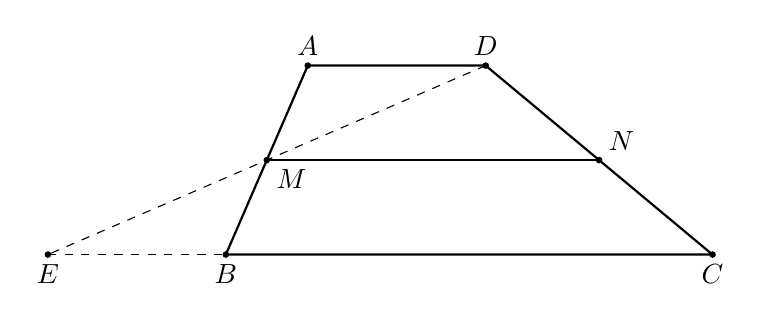
\begin{tikzpicture}[scale=1.0]
  \coordinate (A) at (0,2.4);
  \coordinate (D) at (2.26,2.4);
  \coordinate (B) at (-1.04,0);
  \coordinate (C) at (5.14,0);
  \coordinate (M) at (-0.52,1.2);
  \coordinate (N) at (3.7,1.2);
  \coordinate (E) at (-3.3,0);
  \draw[thick] (A)--(B)--(C)--(D)--cycle;
  \draw[thick] (M)--(N);
  \draw[dashed] (D)--(M)--(E);
  \draw[dashed] (E)--(B);
  \fill (A) circle (1.2pt) node[above] {$A$};
  \fill (D) circle (1.2pt) node[above] {$D$};
  \fill (B) circle (1.2pt) node[below] {$B$};
  \fill (C) circle (1.2pt) node[below] {$C$};
  \fill (M) circle (1.2pt) node[below right] {$M$};
  \fill (N) circle (1.2pt) node[above right] {$N$};
  \fill (E) circle (1.2pt) node[below] {$E$};
\end{tikzpicture}
\end{center}
\nopagebreak[4]
\Needspace{4\baselineskip}
\textbf{解析}

连接 $DM$ 并延长，交 $BC$ 的延长线于点 $E$（见试题卷图）。
\nopagebreak[4]
\begin{center}% 1977 年山西卷第三题：梯形 ABCD（A 左上、D 右上、B 左下、C 右下，上底 AD 短、下底 BC 长），
% M、N 分别为腰 AB、DC 中点，MN 为中位线（实线）；辅助线：DM 延长交 CB 的延长线于 E（虚线 D-M-E），
% E—B 沿底边延长线（虚线）（按源卷第 2 页布局）
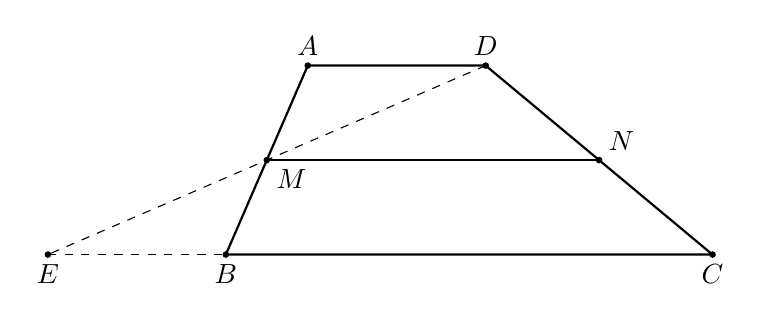
\begin{tikzpicture}[scale=1.0]
  \coordinate (A) at (0,2.4);
  \coordinate (D) at (2.26,2.4);
  \coordinate (B) at (-1.04,0);
  \coordinate (C) at (5.14,0);
  \coordinate (M) at (-0.52,1.2);
  \coordinate (N) at (3.7,1.2);
  \coordinate (E) at (-3.3,0);
  \draw[thick] (A)--(B)--(C)--(D)--cycle;
  \draw[thick] (M)--(N);
  \draw[dashed] (D)--(M)--(E);
  \draw[dashed] (E)--(B);
  \fill (A) circle (1.2pt) node[above] {$A$};
  \fill (D) circle (1.2pt) node[above] {$D$};
  \fill (B) circle (1.2pt) node[below] {$B$};
  \fill (C) circle (1.2pt) node[below] {$C$};
  \fill (M) circle (1.2pt) node[below right] {$M$};
  \fill (N) circle (1.2pt) node[above right] {$N$};
  \fill (E) circle (1.2pt) node[below] {$E$};
\end{tikzpicture}
\end{center}
\nopagebreak[4]
\gksubpart{（1）}

在 $\triangle EBM$ 与 $\triangle DAM$ 中：

$\angle EMB=\angle AMD$（对顶角相等）；

$AM=BM$（$M$ 为 $AB$ 中点，已知）；

$\angle MBE=\angle MAD$（$AD\parallel BC$，即 $AD\parallel BE$，内错角相等）。

\Needspace{5\baselineskip}
由角边角定理，

\nopagebreak[4]
\[
\triangle EBM\cong\triangle DAM\quad(a\text{、}s\text{、}a).
\]

所以 $EM=DM$（对应边相等），$AD=BE$。

\Needspace{5\baselineskip}
又 $DN=NC$（$N$ 为 $DC$ 中点），即 $M\text{、}N$ 分别为 $\triangle DEC$ 边 $DE\text{、}DC$ 的中点，故 $MN$ 为 $\triangle DEC$ 的中位线，所以

\nopagebreak[4]
\[
MN\parallel BC\parallel AD.
\]

\gksubpart{（2）}

\Needspace{5\baselineskip}
由三角形中位线定理，

\nopagebreak[4]
\[
MN=\frac12EC=\frac12(EB+BC)=\frac12(AD+BC).
\]

\gkanswer{答案（1）：见解析版}

\gkanswer{答案（2）：见解析版}

\end{answer}
\begin{answer}
\gksolhead{4}{}

\textbf{题目}（10 分）：

有一块形状为直角三角形的白铁皮，其一直角边和斜边分别为 6 dm 和 10 dm。若从这块白铁皮剪一块最大圆材料，求这圆材料的面积有多大？（$\pi$ 取 3.14）

\Needspace{4\baselineskip}
\textbf{解析}

\Needspace{5\baselineskip}
要从这块白铁皮剪得最大圆材料，此圆必须是直角三角形的内切圆。设内切圆半径为 $r$，直角三角形三边为

\nopagebreak[4]
\[
a=6,\qquad c=10,\qquad b=\sqrt{c^2-a^2}=\sqrt{10^2-6^2}=8.
\]

\Needspace{5\baselineskip}
三角形半周长

\nopagebreak[4]
\[
s=\frac12(6+8+10)=12.
\]

\Needspace{5\baselineskip}
由内切圆半径公式，

\nopagebreak[4]
\[
r=\sqrt{\frac{(s-a)(s-b)(s-c)}{s}}
=\sqrt{\frac{(12-6)(12-8)(12-10)}{12}}
=\sqrt{\frac{6\times4\times2}{12}}=\sqrt4=2.
\]

（用面积法佐证：$r=\dfrac{S_{\triangle}}{s}=\dfrac{\frac12\times6\times8}{12}=2$，一致。）

\Needspace{5\baselineskip}
故内切圆面积

\nopagebreak[4]
\[
\pi r^2\approx3.14\times2^2=12.56\ (\mathrm{dm^2}).
\]

答：剪得的最大圆材料面积约为 $12.56\ \mathrm{dm^2}$。

\gkanswer{答案：约 $12.56\ \mathrm{dm^2}$。}

\end{answer}
\begin{answer}
\gksolhead{5}{}

\textbf{题目}（10 分）：

\Needspace{5\baselineskip}
证明恒等式：

\nopagebreak[4]
\[
\frac{1+\operatorname{Sin}(180^\circ-\alpha)-\operatorname{Cos}(180^\circ+\alpha)+\operatorname{Sin}2\alpha}
{1-\operatorname{Sin}(180^\circ+\alpha)+\operatorname{Cos}(\alpha-360^\circ)}
=\operatorname{Sin}\alpha+\operatorname{Cos}\alpha.
\]

\Needspace{4\baselineskip}
\textbf{解析}

用诱导公式化简两端各项：

分子中 $\sin(180^\circ-\alpha)=\sin\alpha$，$-\cos(180^\circ+\alpha)=-(-\cos\alpha)=+\cos\alpha$，$\sin2\alpha=2\sin\alpha\cos\alpha$；

分母中 $-\sin(180^\circ+\alpha)=-(-\sin\alpha)=+\sin\alpha$，$\cos(\alpha-360^\circ)=\cos\alpha$。

\Needspace{5\baselineskip}
于是左端

\nopagebreak[4]
\[
\text{\text{左边}}
=\frac{1+\sin\alpha+\cos\alpha+2\sin\alpha\cos\alpha}
{1+\sin\alpha+\cos\alpha}.
\]

\Needspace{5\baselineskip}
把分子改写为

\nopagebreak[4]
\[
1+\sin\alpha+\cos\alpha+2\sin\alpha\cos\alpha
=(\sin\alpha+\cos\alpha)^2+(\sin\alpha+\cos\alpha)
=(\sin\alpha+\cos\alpha)(1+\sin\alpha+\cos\alpha),
\]

\Needspace{5\baselineskip}
所以

\nopagebreak[4]
\[
\text{\text{左边}}
=\frac{(\sin\alpha+\cos\alpha)(1+\sin\alpha+\cos\alpha)}
{1+\sin\alpha+\cos\alpha}
=\sin\alpha+\cos\alpha=\text{\text{右边}}.
\]

恒等式成立。

\gkanswer{答案：见解析版}

\end{answer}
\begin{answer}
\gksolhead{6}{}

\textbf{题目}：

$\triangle ABC$ 的三个内角是 $\alpha\text{、}\beta\text{、}\gamma$，而 $\operatorname{tg}\alpha\text{、}\operatorname{tg}\beta$ 是方程 $x^2-5x+6=0$ 的两个根。求 $\gamma$。

\Needspace{4\baselineskip}
\textbf{解析}

\Needspace{5\baselineskip}
因为 $\operatorname{tg}\alpha\text{、}\operatorname{tg}\beta$ 是方程 $x^2-5x+6=0$ 的两个根，由韦达定理，

\nopagebreak[4]
\[
\operatorname{tg}\alpha+\operatorname{tg}\beta=5,\qquad
\operatorname{tg}\alpha\cdot\operatorname{tg}\beta=6.
\]

（事实上两根为 $2\text{、}3$，故 $\alpha\text{、}\beta$ 均为锐角。）

\Needspace{5\baselineskip}
由 $\alpha+\beta+\gamma=180^\circ$，即 $\gamma=180^\circ-(\alpha+\beta)$：

\nopagebreak[4]
\[
\operatorname{tg}\gamma
=\operatorname{tg}\left[180^\circ-(\alpha+\beta)\right]
=-\operatorname{tg}(\alpha+\beta)
=-\frac{\operatorname{tg}\alpha+\operatorname{tg}\beta}
{1-\operatorname{tg}\alpha\operatorname{tg}\beta}
=-\frac{5}{1-6}=1.
\]

又 $\operatorname{tg}(\alpha+\beta)=\dfrac{5}{1-6}=-1<0$，而 $\alpha\text{、}\beta$ 为锐角，故 $\alpha+\beta\in(90^\circ,180^\circ)$，在该范围内正切为 $-1$ 的角唯一，即 $\alpha+\beta=135^\circ$，于是 $\gamma=45^\circ$。

\gkanswer{答案：$\gamma=45^\circ$。}

\end{answer}
\begin{answer}
\gksolhead{7}{}

\textbf{题目}（8 分）：

抛物线的顶点在原点，对称轴为 $y$ 轴，过点 $(1,-1)$，求抛物线方程，焦点坐标，准线方程，开口方向。

\Needspace{4\baselineskip}
\textbf{解析}

\Needspace{5\baselineskip}
因为抛物线的顶点在原点、对称轴为 $y$ 轴，且过点 $(1,-1)$（开口向下），设其标准方程为

\nopagebreak[4]
\[
x^2=-2py\qquad(p>0).
\]

\Needspace{5\baselineskip}
抛物线过点 $(1,-1)$，代入得

\nopagebreak[4]
\[
1^2=-2p\times(-1)
\quad\Longrightarrow\quad
2p=1,\qquad p=\frac12.
\]

\Needspace{5\baselineskip}
因此抛物线的方程为

\nopagebreak[4]
\[
x^2=-y.
\]

\Needspace{5\baselineskip}
焦点坐标为

\nopagebreak[4]
\[
\left(0,-\frac p2\right)=\left(0,-\frac14\right),
\]

\Needspace{5\baselineskip}
准线方程为

\nopagebreak[4]
\[
y=\frac p2=\frac14,
\]

抛物线开口向下。

\gkanswer{答案：$x^2=-y$；焦点 $\left(0,-\dfrac14\right)$；准线 $y=\dfrac14$；开口向下。}

\end{answer}
\begin{answer}
\gksolhead{8}{}

\textbf{题目}（12 分）：

当 $k$ 取何值时，直线 $kx-y-3=0$ 与圆 $2x^2+2y^2-9=0$ 相切，并求出切点坐标。

\begin{gktip}
\textbf{参考题}
\end{gktip}

\textbf{参考题 1．} 已知 $f(x)=x\operatorname{Ln}(2-x)+\sqrt{1+3x^2}$，求 $f'(1)$。

\textbf{参考题 2．} 一水库的水闸为一等腰梯形，上底为 8 米，下底为 4 米，高为 10 米。求当水面与上底相齐时水闸所受的压力。（已知水的比重为 1 吨重/立方米）

\begin{gktip}
原源 PDF 第 4 页附有水闸（倒梯形）与水深 $x$ 处面积元示意图；LaTeX 版按源图重绘。
\end{gktip}
\nopagebreak[4]
\begin{center}% 1977 年山西卷参考题 2：水库水闸（等腰梯形，上底 8 米、下底 4 米、高 10 米），
% 水面与上底相齐（顶部水平线为水面线）；水深 x 米处取水平面积元（阴影条，高 dx），
% 左侧标 x 米（水面到面积元的深度）、右侧标总高 10 米、底部标下底 4 米（按源卷第 4 页布局）
\begin{tikzpicture}[scale=0.86,>=stealth]
  % 水闸（倒梯形：上底宽、下底窄）
  \coordinate (TL) at (0,3);
  \coordinate (TR) at (5,3);
  \coordinate (BL) at (1,0);
  \coordinate (BR) at (4,0);
  \draw[thick] (TL)--(BL)--(BR)--(TR)--cycle;
  % 水面线（与上底相齐，两端延伸）
  \draw[thick] (-0.5,3)--(5.7,3);
  % 深度 x 处的水平面积元（阴影条，高 dx）
  \draw (0.72,2.15) rectangle (4.28,2.35);
  \foreach \x in {0.85,1.15,...,4.05}{
    \draw (\x,2.15)--(\x+0.2,2.35);
  }
  \node[right] at (4.55,2.25) {$dx$};
  % 左侧：x 米（水面到面积元）
  \draw[<->] (-0.25,3)--(-0.25,2.15);
  \node[left,rotate=90,anchor=center] at (-0.42,2.6) {$x\,\text{米}$};
  % 右侧：总高 10 米
  \draw[<->] (5.45,3)--(5.45,0);
  \node[right,rotate=90,anchor=center] at (5.62,1.5) {$10\,\text{米}$};
  % 底部：下底 4 米
  \draw[<->] (1,-0.4)--(4,-0.4);
  \node[below] at (2.5,-0.45) {$4\,\text{米}$};
  % 顶部：上底 8 米
  \draw (0,3.12)--(0,3.3);
  \draw (5,3.12)--(5,3.3);
  \draw[<->] (0,3.25)--(5,3.25);
  \node[above] at (2.5,3.28) {$8\,\text{米}$};
\end{tikzpicture}
\end{center}
\nopagebreak[4]
\Needspace{4\baselineskip}
\textbf{解析}

\Needspace{5\baselineskip}
把直线 $y=kx-3$ 代入圆方程 $2x^2+2y^2-9=0$：

\nopagebreak[4]
\[
2x^2+2(kx-3)^2-9=0,
\]

\Needspace{5\baselineskip}
整理得

\nopagebreak[4]
\[
2(k^2+1)x^2-12kx+9=0.
\]

\Needspace{5\baselineskip}
直线与圆相切等价于此二次方程有两相等实根，即判别式为零：

\nopagebreak[4]
\[
\Delta=(12k)^2-4\times2(k^2+1)\times9
=144k^2-72(k^2+1)
=72(k^2-1)=0,
\]

所以 $k^2=1$，即 $k=\pm1$。

\Needspace{5\baselineskip}
切点即重合的交点，由求根公式（重根）

\nopagebreak[4]
\[
x=\frac{12k}{2\times2(k^2+1)}=\frac{3k}{k^2+1},
\qquad
y=kx-3.
\]

$k=1$ 时：$x=\dfrac32$，$y=\dfrac32-3=-\dfrac32$，切点为 $\left(\dfrac32,-\dfrac32\right)$；

$k=-1$ 时：$x=-\dfrac32$，$y=\dfrac32-3=-\dfrac32$，切点为 $\left(-\dfrac32,-\dfrac32\right)$。

（与源解答写出的交点坐标公式 $x=\dfrac{6k\pm3\sqrt{2(k^2-1)}}{2(k^2+1)}$、$y=\dfrac{-6\pm3k\sqrt{2(k^2-1)}}{2(k^2+1)}$ 在 $2(k^2-1)=0$ 时的结果一致。）

\textbf{参考题 1}

\Needspace{5\baselineskip}
由乘积与商的求导法则，

\nopagebreak[4]
\[
f'(x)=\bigl[x\ln(2-x)\bigr]'+\bigl[\sqrt{1+3x^2}\bigr]'
=\ln(2-x)+x\cdot\frac{-1}{2-x}+\frac{6x}{2\sqrt{1+3x^2}},
\]

\Needspace{5\baselineskip}
即

\nopagebreak[4]
\[
f'(x)=\ln(2-x)-\frac{x}{2-x}+\frac{3x}{\sqrt{1+3x^2}}.
\]

\Needspace{5\baselineskip}
所以

\nopagebreak[4]
\[
f'(1)=\ln1-\frac{1}{2-1}+\frac{3}{2}
=0-1+\frac32=\frac12.
\]

\textbf{参考题 2}
\nopagebreak[4]
\begin{center}% 1977 年山西卷参考题 2：水库水闸（等腰梯形，上底 8 米、下底 4 米、高 10 米），
% 水面与上底相齐（顶部水平线为水面线）；水深 x 米处取水平面积元（阴影条，高 dx），
% 左侧标 x 米（水面到面积元的深度）、右侧标总高 10 米、底部标下底 4 米（按源卷第 4 页布局）
\begin{tikzpicture}[scale=0.86,>=stealth]
  % 水闸（倒梯形：上底宽、下底窄）
  \coordinate (TL) at (0,3);
  \coordinate (TR) at (5,3);
  \coordinate (BL) at (1,0);
  \coordinate (BR) at (4,0);
  \draw[thick] (TL)--(BL)--(BR)--(TR)--cycle;
  % 水面线（与上底相齐，两端延伸）
  \draw[thick] (-0.5,3)--(5.7,3);
  % 深度 x 处的水平面积元（阴影条，高 dx）
  \draw (0.72,2.15) rectangle (4.28,2.35);
  \foreach \x in {0.85,1.15,...,4.05}{
    \draw (\x,2.15)--(\x+0.2,2.35);
  }
  \node[right] at (4.55,2.25) {$dx$};
  % 左侧：x 米（水面到面积元）
  \draw[<->] (-0.25,3)--(-0.25,2.15);
  \node[left,rotate=90,anchor=center] at (-0.42,2.6) {$x\,\text{米}$};
  % 右侧：总高 10 米
  \draw[<->] (5.45,3)--(5.45,0);
  \node[right,rotate=90,anchor=center] at (5.62,1.5) {$10\,\text{米}$};
  % 底部：下底 4 米
  \draw[<->] (1,-0.4)--(4,-0.4);
  \node[below] at (2.5,-0.45) {$4\,\text{米}$};
  % 顶部：上底 8 米
  \draw (0,3.12)--(0,3.3);
  \draw (5,3.12)--(5,3.3);
  \draw[<->] (0,3.25)--(5,3.25);
  \node[above] at (2.5,3.28) {$8\,\text{米}$};
\end{tikzpicture}
\end{center}
\nopagebreak[4]
\Needspace{5\baselineskip}
压力、压强与面积的关系为 $F=PS$。由物理学知识，水面以下 $x$ 米处的压强等于深度与水的比重的乘积：

\nopagebreak[4]
\[
P=x\cdot1=x\ (\text{\text{吨重}/\text{平方米}}).
\]

\Needspace{5\baselineskip}
水闸为等腰梯形，上底 8 米、下底 4 米、高 10 米，水面与上底相齐。由相似三角形（线性插值），水深 $x$ 米处的水平线段长为

\nopagebreak[4]
\[
\ell(x)=8-\frac{8-4}{10}x=8-\frac25x.
\]

\Needspace{5\baselineskip}
取高为 $dx$ 的水平面积元，此面积元所受压力

\nopagebreak[4]
\[
dF=P\,\ell(x)\,dx=x\left(8-\frac25x\right)dx.
\]

\Needspace{5\baselineskip}
因此总压力

\nopagebreak[4]
\[
F=\int dF=\int_0^{10}x\left(8-\frac25x\right)dx
=\left.\left(4x^2-\frac{2x^3}{15}\right)\right|_0^{10}
=400-\frac{400}{3}=\frac{800}{3}\ (\text{\text{吨}}).
\]

答：水闸所受的压力为 $\dfrac{800}{3}$ 吨。

\gkanswer{答案：$k=\pm1$；切点 $\left(\dfrac32,-\dfrac32\right)$ 与 $\left(-\dfrac32,-\dfrac32\right)$。}

\end{answer}